\documentclass{report}
\usepackage{listings}
\usepackage[margin=1.0in]{geometry}
\usepackage{graphicx}
\usepackage{hyperref}
\usepackage{amsmath}
\hypersetup{colorlinks=true}
\usepackage[document]{}
\title{EECE.5200 - Homework 3}
\author{Travis Kessler}
\date{9 March 2021}
\begin{document}
	\maketitle
	\newpage

	% \lstset{language=shell}
	\lstset{frame=lines}

	\section*{Accessing Source Code}
	
	Source code is available at: \href{https://github.com/tjkessler/eece5200/tree/main/hw3}{https://github.com/tjkessler/eece5200/tree/main/hw3}
	
	\textit{}
	
	\noindent To run the code, first run \textbf{\textit{make}} in the "hw3" directory. This will produce X files: "q1j.o", "q1gs.o", "q2.o", "q3.o", and "q4.0". The resulting files can be executed from the command line. An additional script written in Python is included for plotting Jacobi iteration and Gauss-Siedel iteration convergence errors after their executables are run. To display the gnuplot showing results for question 4, execute \textbf{\textit{gnuplot -persistent question\_4.gnu}}.
	
	\section*{Question 1}
	
	\subsection*{a.}
	
	Given the differential equation
	
	\textit{}
	
	$\frac{d^2y}{dx^2} + 3 \frac{dy}{dx} + 2y = 0$

	\textit{}
	
	\noindent evaluated over the interval $0 \leq x \leq 1$ with boundary conditions $y(0) = 1.0$ and $y(1) = 2.0$, the equation $y$ can be assumed to have a solution in the form of $e^{\lambda x}$:
	
	\textit{}
	
	$\left( e^{\lambda x} \right) '' + 3 \left( e^{\lambda x} \right) + 2e^{\lambda x}$
	
	\textit{}
	
	\noindent which is simplified to
	
	\textit{}
	
	$e^{\lambda x} \left( \lambda^2 + 3 \lambda + 2 \right) = 0$
	
	\textit{}
	
	\noindent Solving for $\lambda$, which equals $-1$ and $-2$, we find that
	
	\textit{}
	
	$y(x) = c_1 e^{-x} + c_2 e^{-2x}$
	
	\textit{}
	
	\noindent Given the boundary conditions $y(0) = 1.0$ and $y(1) = 2.0$, we can solve for $c_1$ and $c_2$:
	
	\textit{}
	
	$y(0) = 1 = c_1 e^0 + c_2 e^0$
	
	$\rightarrow c_1 = 1 - c_2$
	
	\textit{}
	
	$y(1) = 2 = c_1 e^{-1} + c_2 e^{-2}$
	
	$\rightarrow c_1 = 2e^2 - c_2 e$
	
	\textit{}
	
	\noindent Solving for $c_1$ and $c_2$, we find that
	
	\textit{}
	
	$y = \frac{1 - 2e^2}{1 - e} e^{-x} - \frac{2e^2 - e}{1 - e} e^{-2x} \approx 8.0185e^{-x} - 7.0185e^{-2x}$
	
	\textit{}
	
	\newpage
	
	\subsection*{b.}
	
	Given that $x_j = j \partial x$, $y(x_j) = y_j$, $\partial x = \frac{1}{N}$ where $j = (0, N)$, and $N = 10$:
	
	\textit{}
	
	$\frac{d^2 y}{dx^2} = \frac{y_{j - 1} - 2y_j + y_{j + 1}}{(\partial x)^2} = 100 \left( y_{j - 1} -2y_j + y_{j + 1} \right)$
	
	\textit{}
	
	$\frac{dy}{dx} = \frac{y_{j + 1} - y_{j - 1}}{2 \partial x} = 5 \left( y_{j + 1} - y_{j - 1} \right)$
	
	\textit{}
	
	\noindent These equalities can then be substituted into the original differential equation:
	
	\textit{}
	
	$0 = 100 \left( y_{j - 1} -2y_j + y_{j + 1} \right) + 15 \left( y_{j + 1} - y_{j - 1} \right) + 2y_j$
	
	\textit{}
	
	\noindent Solving for $y_j$:
	
	\textit{}
	
	$y_j = \frac{85}{198} y_{j - 1} + \frac{115}{198} y_{j + 1} \approx 0.4292y_{j - 1} + 0.5808y_{j + 1}$
	
	\textit{}
	
	\subsection*{c. \& d.}
	
	Figure 1 compares the abilities of the Jacobi iteration method (\textit{question\_1\_jacobi.c}) and the Gauss-Siedel iteration method (\textit{question\_1\_gauss\_siedel.c}) when applied to the above differential equation. An error threshold of $0.0001$ was used as a cutoff. It is apparent that while the Gauss-Siedel iteration method has a higher error at the beginning of the iteration process, it converges much quicker (26 iterations) compared to the Jacobi iteration method (49 iterations). Note that a value of $N = 5$ was used for this experiment; other values, such as $N = 10$, do not allow convergence of this specific differential equation (Figure 2).
	
	\begin{figure}[!ht]
		\centering
		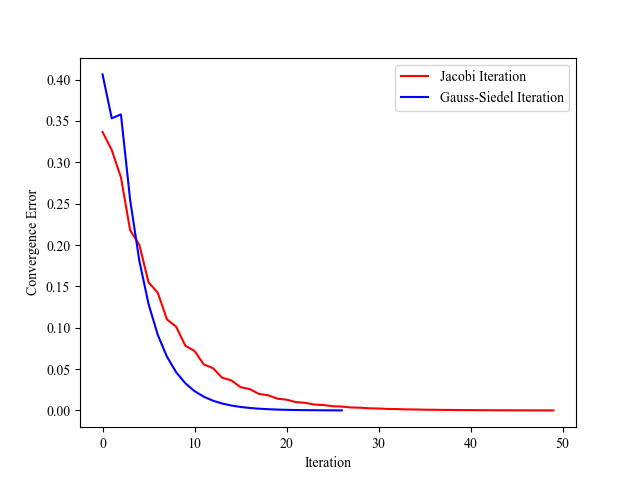
\includegraphics[scale=0.9]{figures/convergence_curve.png}
		\caption{Comparison of convergence between Jacobi iteration and Gauss-Siedel iteration, N = 5}
	\end{figure}

	\begin{figure}[!ht]
		\centering
		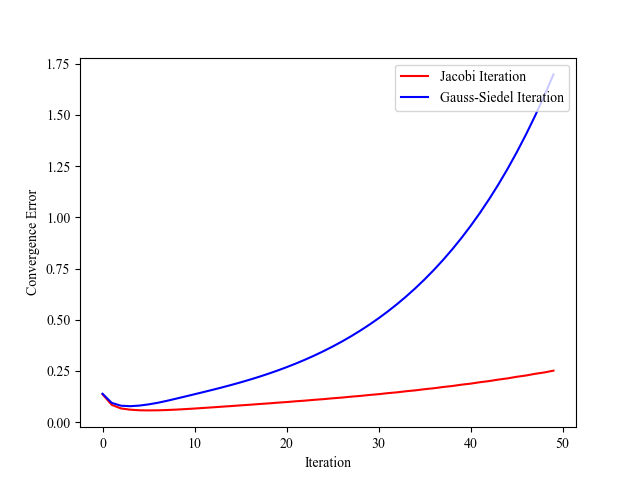
\includegraphics[scale=0.9]{figures/convergence_curve_bad.png}
		\caption{Comparison of convergence between Jacobi iteration and Gauss-Siedel iteration, N = 10}
	\end{figure}

	\section*{Question 2}
	
	Upon executing "q2.o", the following console output was achieved:
	
	\begin{lstlisting}
((base) tjkessler@Traviss-MacBook-Air hw3 % ./q2.o
Eigenvalues:
1  -1.00000048       0.00000000    
2  -1.99999642       0.00000000    
3  -3.00000310       0.00000000    

Eigenvectors:
1                2                 3
0.577350020     -0.462912798      -1.87081456    
-0.577350378      0.925823867       5.61244488    
0.577350616      -1.85164404      -16.8373451    

State Transition Matrix:
1    e^(  -1.00000048     *t)
2    e^(  -1.99999642     *t)
3    e^(  -3.00000310     *t)

y(t) = 
+ (450.001556,0.00000000)  * e^((-1.00000048,0.00000000) *t)
+ (-640.000366,0.00000000)  * e^((-1.99999642,0.00000000) *t)
+ (209.998779,0.00000000)  * e^((-3.00000310,0.00000000) *t)
	\end{lstlisting}

	\section*{Question 3}
	
	Upon executing "q3.o", the following console output was achieved:
	
	\begin{lstlisting}
(base) tjkessler@Traviss-MacBook-Air hw3 % ./q3.o
Eigenvalues:
1  0.801336944    
2  0.798662126    
3   62830.0977    

Eigenvectors:
1                2                 3
-1.05343270      -7.53999688E-03   2.22724104    
-331.687622       2.36182666      -1.33629358    
3.18041658       2.24758890E-02   1.67039597    

State transition matrix:
1  -7.64506757E-02  -1.20494980E-03  0.100972421    
2  -10.5383492      0.169503137       14.1870241    
3   22568.0957      0.457639933       7522.83936 
	\end{lstlisting}

	\section*{Question 4}
	
	Upon executing "q4.o", the following console output was achieved:

	\begin{lstlisting}
(base) tjkessler@Traviss-MacBook-Air hw3 % ./q4.o 
=== NO DIMENSIONALITY REDUCTION ===
COEFFICIENTS:
1  -37176.9570    
2   366.118469    
3 -0.895457685    
PREDICTIONS:
1   59.5292969       75.0000000       190.000000    
2   84.4765625       91.0000000       191.000000    
3   107.640625       105.000000       192.000000    
4   129.007812       122.000000       193.000000    
5   148.582031       131.000000       194.000000    
6   166.367188       150.000000       195.000000    
7   182.359375       179.000000       196.000000    
8   196.562500       203.000000       197.000000    
9   208.972656       227.000000       198.000000    
10   219.601562       249.000000       199.000000    
11   228.429688       281.000000       200.000000    
RMSE, fitting set:    11.9847345    
RMSE, testing set:    141.061218    

=== SMALLEST SINGULAR VALUE REMOVED ===
COEFFICIENTS:
1 -0.177643716    
2  -17.2275963    
3   9.25780535E-02
PREDICTIONS:
1   68.6464844       75.0000000       190.000000    
2   86.6914062       91.0000000       191.000000    
3   104.921143       105.000000       192.000000    
4   123.336182       122.000000       193.000000    
5   141.936279       131.000000       194.000000    
6   160.721436       150.000000       195.000000    
7   179.691895       179.000000       196.000000    
8   198.847412       203.000000       197.000000    
9   218.188232       227.000000       198.000000    
10   237.714111       249.000000       199.000000    
11   257.425049       281.000000       200.000000    
RMSE, fitting set:    6.58823967    
RMSE, testing set:    164.580048 
	\end{lstlisting}

\noindent It is observed that when the smallest singular value is removed from the Sigma matrix resulting from SVD, the fitting/training prediction root mean-squared error is smaller, but the test prediction root mean-squared error is larger. The larger test error can likely be attributed to a small sample size, and would not be representative of a larger test set; realistically it is lower than the full-valued SVD's test error. This is apparent in Figure 3, where predictions using the SVD with its smallest singular value removed trend closer to the actual data.

\begin{figure}[!ht]
	\centering
	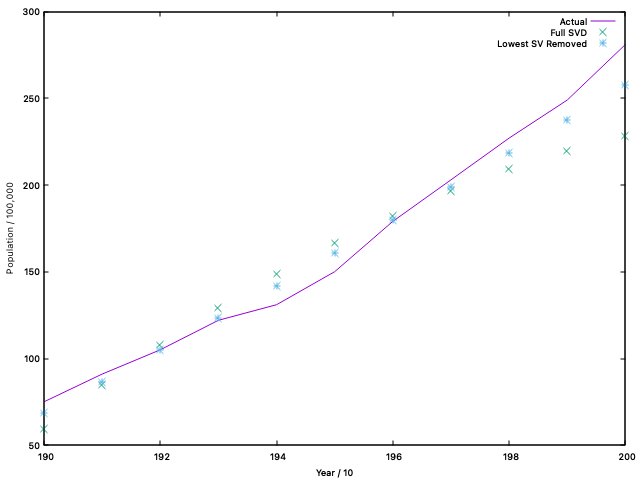
\includegraphics[scale=0.7]{figures/q4_results.png}
	\caption{Comparison between actual data, SVD LSR with all singular values, SVD LSR without lowest singular value}
\end{figure}

	\begin{thebibliography}{99\kern\bibindent}
	
	\bibitem{hwref}
	Thompson, C.
	\textit{University of Massachusetts Lowell Department of Electrical and Computer Engineering 16.520 Computer Aided Engineering Analysis Problem Set 3}.
	Retrieved March 9, 2021, from http://morse.uml.edu/Activities.d/16.520/S2021.d/HW3.pdf
	
	\end{thebibliography}

\end{document}